\section{Theory}
We will not try to derive the whole electroweak theory again. Here only some important, relevant equations are presented.

\paragraph{Decay width}
The partial decay width of $Z^0$ decay into fermion $f$ is~\cite{manual}
\begin{equation}
	\Gamma_f = \frac{ \sqrt{2} N_c^f}{12\pi} G_F M_Z^3 \left( (g_V^f)^2 + (g_A^f)^2  \right)
	\label{math:Gammaf}
\end{equation}
with
\begin{align*}
	g_V^f &= I_3^f - 2 Q_f \sin^2 \theta_W \\
	g_A^f &= I_3^f 
\end{align*}
One needs to be aware that $\Gamma_f$ contains contribution from both chiralities, and $I_3$ here refers to only the weak isospin of left-handed fermions (by definition right handed fermions have no weak isospin).

Partial cross section of $Z^0 \rightarrow f\bar{f}$ is given by~\cite{manual}
\begin{equation}
	\sigma_f(s) = \frac{12 \pi}{M_Z^2} \frac{s \Gamma_e \Gamma_f}{ (s-M_Z^2)^2 + (s^2 \Gamma^2_Z / M_Z^2)}
	\label{math:sigmaf}
\end{equation}
and exactly at peak of resonance
\begin{equation}
	\sigma_{f, \text{peak}} = \frac{12 \pi}{M_Z^2} \frac{\Gamma_e \Gamma_f}{\Gamma_Z^2}
	\label{math:sigmafPeak}
\end{equation}

\paragraph{Angular distribution}
In $ee \rightarrow ee$ scattering, two relevant channels have different angular dependences. For $s$-channel~\cite{manual},
\begin{equation}
	\dv{\sigma}{\Omega}_s \sim (1 + \cos^2 \Theta)
	\label{math:diffCrossS}
\end{equation}
For $t$-channel,
\begin{equation}
	\dv{\sigma}{\Omega}_t \sim (1-\cos^2 \Theta)^{-2}
	\label{math:diffCrossT}
\end{equation}


\paragraph{Forward-Backward Asymmetry} is defined as 
\begin{equation}
	A_{FB} = \frac{N_+ - N_-}{N_+ + N_-}
	\label{math:AFBdef}
\end{equation}
where $N_{+,-}$ denotes number of events in forward or backward direction.

Near $Z^0$ resonance can be approximated by~\cite{manual}
\begin{align}
	\begin{split}
	A_\text{FB}^f &\approx \frac{-3}{2} \frac{a_e a_f Q_f \Re(\chi)}{(v_e^2 + a_e^2) (v_f^2 + a_f^2)} \\
	&=  \frac{-3}{2} \frac{a_e a_f Q_f }{(v_e^2 + a_e^2) (v_f^2 + a_f^2)} \frac{s(s-M_Z^2)}{(s-M_Z^2)^2 + (s \Gamma_Z / M_Z)^2 }
	\end{split}
	\label{math:AFBgen}
\end{align}
Exactly at resonance peak, we have
\begin{equation}
	A_\text{FB}^{l,\text{peal}} \approx 3 \left( \frac{v_l}{a_l} \right)^2 = 3 \left( \frac{I_3^l - 2 Q_l \sin^2\theta_W}{I_3^l} \right)^2
	\label{math:AFBpeak}
\end{equation}

\paragraph{The OPAL-Detector}
We have used data in this experiment from OPAL detector. OPAL was one of the four detector devices at LEP at the CERN \cite{manual}. The collision point is surrounded by an central detector with  a vertex chamber, jet- and Z-chambers. The main function of all these chambers is tracking the charged particles. The whole device is situated within an autoclave contains a mixture of argon, methane and isobutane at a pressure of 4 bar \cite{manual}.

The central detector is surrounded by two calorimeters: electromagnetic calorimeter (ECAL) and hadronic calorimeter (HCAL). ECAL consists of lead glass blocks and surrounding jet chamber. The cathod pads are arranged behind these blocks. The energy and position of the electromagnetic showers are determined by th signal from cathode pads. The electron-positron particle showers deposited their energy in ECAL. Hadrons deposited their some part of energy in ECAL and rest of the part in HCAL. 

Whole set up surrounded by draft chamber where charged particles usually muons are detected, therefore it is called muons chamber. A Forward Calorimeter (FCAL) is arranged close to the beam pipe consist of a sandwich of lead glass. FCAL used to measured the luminosity.


\begin{figure}[H]
	\centering
	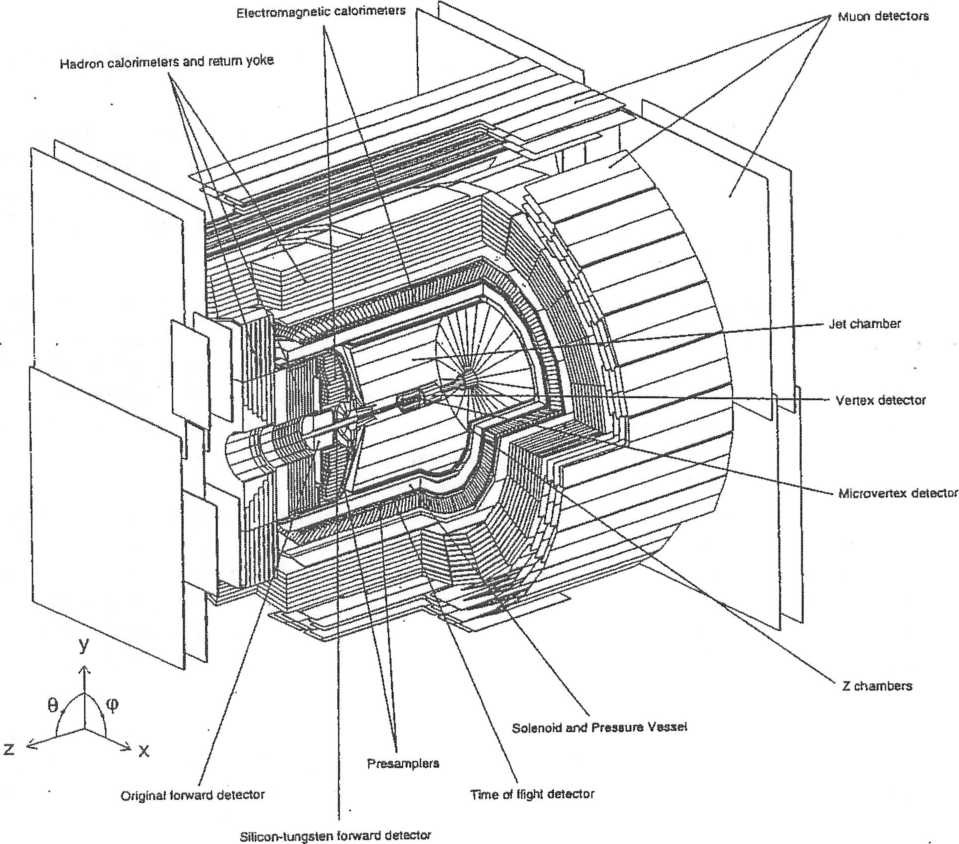
\includegraphics[width=0.8\linewidth]{opal.jpg}
	\caption{ The OPAL detector \cite{manual}. }
	\label{fig:OPAL}
\end{figure}
